\documentclass{rapport}
\usepackage{lipsum}
%\usepackage{gensymb}
\usepackage{float}
\usepackage{graphicx} % Required for inserting images
\usepackage{amsfonts}
\usepackage{wrapfig}
\usepackage{afterpage}
\usepackage{amsmath,amssymb}
\usepackage[ruled,vlined]{algorithm2e}
\usepackage{url}

\usepackage{pgfplots}
\pgfplotsset{compat=1.18}
\usetikzlibrary{arrows.meta} % For nicer arrows


\usepackage{tcolorbox}
\tcbuselibrary{theorems, skins}  


\definecolor{maincolor}{HTML}{1E90FF}


\SetKwSty{textcolor{maincolor}}
\SetArgSty{textcolor{maincolor}}
\SetCommentSty{textcolor{maincolor}}


\newtcbtheorem{teorema}{Teorema}%
{colback=maincolor!10!white,
 colframe=maincolor!80!black,
 fonttitle=\bfseries,
 coltitle=black,
 boxrule=0.8pt,
 arc=4pt,
 enhanced}{th}




\definecolor{vscodeBlue}{RGB}{4,100,179}       % keywords
\definecolor{vscodeRed}{RGB}{170,0,0}      % strings
\definecolor{vscodeGreen}{RGB}{0,128,0}      % comments
\definecolor{vscodeDarkYellow}{RGB}{242,134,29} % function names / identifiers
\definecolor{vscodePurple}{RGB}{0,0,110}   % numbers

% Setup listings for Python
\lstset{
    language=Python,
    keywordstyle=\color{vscodeBlue}\bfseries,
    stringstyle=\color{vscodeRed},
    commentstyle=\color{vscodeGreen}\itshape,
    identifierstyle=\color{vscodeDarkYellow},
    numbers=left,
    numberstyle=\tiny\color{gray},
    numbersep=5pt,
    backgroundcolor=\color{white},  % white background
    showstringspaces=false,
    basicstyle=\ttfamily\small,
    breaklines=true,
    frame=tb,
}



\title{Crittografia} %title of the file

\begin{document}

%----------- Report information ---------

\logo{logos/logo.jpg}
\uni{\textbf{Newton-Pertini di Camposampiero}}
\ttitle{Crittografia} %title of the file
\subject{Sistemi e Reti} % Subject name
\topic{Crittografia} % Topic name

\professor{Gianfranco \textsc{Lamon}} % information related to the professor

\students{Alex Gasparini} % information related to the students

%----------- Init -------------------
        
\buildmargins % display margins
\buildcover % create the front cover of the document
\toc % creates the table of contents

%------------ Report body ----------------

\section{Introduzione}

In questo corso andremo a vedere le basi della \textbf{Crittografia moderna}. In primis, dobbiamo capire cosa vuol dire “\textit{Crittografia}”. Partiamo dall’etimologia: dal greco \textbf{\textit{kryptós}} (nascosto) – \textbf{\textit{graphía}} (scrittura). In sostanza, la Crittografia è la disciplina che studia e analizza come inviare e ricevere messaggi \textbf{nascosti}. Con il termine “nascosti” si intende che solo ed esclusivamente la sorgente e il destinatario possono leggere il contenuto del messaggio, mentre qualsiasi altra persona non può.

\begin{figure}[h]
     \centering
    \includegraphics[width=0.6\linewidth]{logos/0_1_cripto.pdf}
\end{figure}

In questa immagine l'utente A manda un messaggio criptato all’utente B; in questo modo solo A e B potranno leggere il contenuto del messaggio, mentre l’intercettatore, anche se riuscisse ad averne una copia, non sarebbe in grado di leggerlo (dato che è criptato).

La crittografia la usiamo tutti i giorni (anche involontariamente) con i nostri dispositivi elettronici. Un esempio è \textbf{WhatsApp}, che tramite una crittografia \textbf{End-to-End} (che avremo tempo di approfondire) permette di inviare messaggi in maniera sicura, in modo che nessun altro (nemmeno WhatsApp stesso!) possa leggere il messaggio che hai mandato al tuo amico. Ha anche utilità nell’autenticazione digitale e nei documenti elettronici: infatti, tutti i sistemi come \textbf{SPID} oppure \textbf{CIE} sfruttano la crittografia per funzionare. La crittografia viene utilizzata anche dalle case produttrici di console (come \textbf{Sony} per la \textbf{PlayStation}) per impedire di crackare le loro console. Di esempi ce ne sono a centinaia e avremo tempo per scoprirli tutti.


Anche se ho elencato molti esempi \textbf{digitali}, la crittografia è una disciplina basata sulla \textbf{matematica}. Infatti, tutti i sistemi crittografici si fondano su prove matematiche (come il \textbf{Logaritmo Discreto} e la \textbf{Fattorizzazione di numeri composti}) per funzionare. Mi piace definire la crittografia come una branca a metà strada tra matematica e informatica, poiché utilizza concetti matematici applicati a contesti informatici.

\newpage

Un altro punto fondamentale da chiarire è che, anche se parleremo di sistemi moderni come \textbf{AES}, \textbf{RSA}, \textbf{Diffie-Hellman} e \textbf{ECC}, inventati tra il 1960 e il 1990 circa, in realtà la crittografia è molto più antica. Già dall’\textbf{Impero Romano} (753 a.C. – 476 d.C.) se ne parlava: chiaramente i sistemi erano molto più semplici di quelli odierni, ma all’epoca servivano per inviare messaggi all’esercito. In questo coro di cifrari "antichi" ne vedremo due, forse i più impattanti nella storia: il \textbf{Cifrario di Cesare}, che possiamo definire il primo sistema crittografico, e la macchina \textbf{Enigma}, che durante la Seconda Guerra Mondiale fu di fondamentale importanza per le truppe dell’Asse; gli alleati, grazie a \textbf{Alan Turing}, riuscirono a decifrarla, aiutando così la loro vittoria.

Fatte tutte le premesse del caso, iniziamo a parlare di crittografia; come prima cosa, vediamo e definiamo tutti i termini utilizzati in questo ambito.


\subsubsection{Cifratura} 

La cifratura di un messaggio è il processo che permette di \textbf{alterare} un messaggio in modo che nessun altro (eccetto chi lo invia e il destinatario) possa leggere il contenuto originario. La cifratura deve avvenire tramite un \textbf{algoritmo di cifratura} e con l’ausilio di una (o più) \textbf{chiavi}.


\begin{figure}[h]
     \centering
    \includegraphics[width=0.8\linewidth]{logos/0_2_cripto.pdf}
\end{figure}

In questo caso, il messaggio "\textbf{Ciao sono Alex}" tramite una cifratura è diventato \textbf{-QnbB\^{}DUxQxUP\^{}}; se qualcuno riuscisse a intercettare il messaggio cifrato, non capirebbe nulla.


\subsubsection{Decifratura} 

La decifratura è il passaggio \textbf{inverso} della cifratura, nel senso che permette di tornare al messaggio originale partendo dal messaggio cifrato. Chiaramente, bisogna usare lo \textbf{stesso algoritmo di cifratura} e, soprattutto, la \textbf{stessa chiave}, che deve essere conosciuta solo da chi invia il messaggio e da chi lo deve ricevere.


\begin{figure}[h]
     \centering
    \includegraphics[width=0.8\linewidth]{logos/0_3_cripto.pdf}
\end{figure}

\newpage

Iniziamo a utilizzare un po' di nozionismo matematico: il meccanismo di cifratura e decifratura può essere paragonato a una \textbf{funzione}, poiché entrambe prendono una variabile in input e restituiscono un valore in output. Possiamo quindi definire la cifratura come


\begin{equation*}
    c = f(m)
\end{equation*}

Dove $c$ è il messaggio cifrato, $m$ è il messaggio originale e $f$ è la “funzione di cifratura”. Dato ciò, la “funzione di decifratura” sarà definita come


\begin{equation*}
    m = f^{-1}(c)
\end{equation*}

Questo può essere dedotto dalla seguente equazione:


\begin{equation*}
    m = f^{-1}(f(m)) 
\end{equation*}

Tranquilli, per ora abbiamo terminato con il nozionismo matematico.


\subsubsection{Chiave} 

Una chiave è una qualsiasi \textbf{stringa} o, più semplicemente, un \textbf{numero}; la caratteristica principale è che una chiave deve \textbf{rimanere privata}, perché permette di cifrare e decifrare i messaggi. Se qualcuno riuscisse a rintracciare la vostra chiave privata, potrebbe leggere tutti i messaggi che inviate e ricevete. L’idea della chiave in crittografia è simile a quella di una \textbf{password}: allo stesso modo, se qualcuno vi ruba la password, può accedere al vostro account. In realtà, la chiave può anche essere qualcosa di più complesso, come un \textbf{punto nel piano cartesiano} (usato nella \textit{Elliptic Curve Cryptography}).

Quindi, per evitare confusione, correggiamo la definizione precedente dicendo che una chiave è un qualsiasi \textbf{dato}, oppure un \textbf{insieme di dati}, che deve rimanere \textbf{segreto}.

In realtà, vedremo verso metà corso che esiste anche una cosiddetta \textbf{chiave pubblica}, ovvero una chiave come quella che abbiamo definito fino a ora, ma che \textbf{chiunque può conoscere}. Se vi sembra strano o controintuitivo, quando lo vedremo tutto sarà chiaro.


\subsubsection{Rotto} 

Un sistema crittografico si definisce \textbf{rotto} qualora sia possibile decifrare un messaggio criptato senza conoscere la chiave. Un sistema rotto, chiaramente, non può essere utilizzato, perché chiunque riuscirebbe a decifrare il messaggio. Un esempio di sistema rotto è il \textbf{DES} (che vedremo nel capitolo “Cifrari a Blocchi”). Il DES è stato inventato nel 1976 e, all’inizio, era molto usato; il problema era che utilizzava una chiave a lunghezza fissa: 54 bit. Ad oggi, purtroppo, una chiave a 54 bit è soggetta ad attacchi \textbf{brute-force}\footnote{Attacchi in cui si provano tutte le possibili combinazioni di una chiave; richiedono molto tempo, ma per chiavi molto piccole (come il DES) possono funzionare}, e per questo oggi il DES non può più essere usato per cifrare ed è stato sostituito dall’\textbf{AES}.


\newpage





\subsection{Principio di Kerckhoffs}

Ora che abbiamo iniziato a familiarizzare con i primi termini della crittografia, possiamo comprendere il principio fondante della disciplina: il \textbf{Principio di Kerckhoffs}.


\begin{teorema}{Principio di Kerckhoffs}{}
La sicurezza di un sistema crittografico deve dipendere unicamente dalla chiave segreta e non dalla segretezza dell’algoritmo stesso.

\end{teorema}

Sostanzialmente, Kerckhoffs afferma che non deve essere segreto \textbf{l’algoritmo di cifratura}; la forza di un sistema crittografico deriva invece dalla difficoltà di romperlo, e non dalla segretezza dell’algoritmo.


Per questo motivo, oggi sappiamo perfettamente quali algoritmi utilizzano i vari siti e le app; non è un rischio conoscere il metodo con cui viene criptato un messaggio, perché la sicurezza risiede nella segretezza della chiave, che, chiaramente, deve rimanere privata. 


Per esempio, secondo Kerckhoffs, se tu e un tuo amico volete creare un sistema per scambiarvi messaggi segreti, non potete semplicemente utilizzare un sistema debole mantenendolo segreto a tutti gli altri; se qualcuno riuscisse a scoprire l’algoritmo, potrebbe leggere tutti i vostri messaggi. i messaggi.





\subsection{Il problema dello scambio della Chiave}

Prima di cominciare a parlare della classificazione dei sistemi crittografici, è necessario affrontare il problema dello scambio della chiave. Ripetendo quanto visto finora, la crittografia studia come due utenti possano scambiarsi messaggi in modo che nessun altro ne possa leggere il contenuto. Abbiamo capito che il messaggio viene cifrato e poi decifrato tramite un algoritmo. Inoltre, un algoritmo ha bisogno di una chiave per cifrare i messaggi, e la chiave deve essere posseduta solo da chi invia il messaggio e da chi lo deve ricevere; nessun altro dovrebbe conoscerla, altrimenti anche altri utenti potrebbero decifrare i messaggi. Tuttavia, non abbiamo ancora considerato come i due utenti possano scambiarsi una chiave comune o, comunque, concordare su una chiave da usare nel sistema.


\begin{figure}[h]
    \centering
    \includegraphics[width=0.6\linewidth]{logos/0_5_cripto.pdf}
\end{figure}

In questa immagine, l’utente A ha generato una chiave da usare per cifrare i messaggi, ma deve trovare un modo per inviarla a B (così che lui possa decifrare i messaggi di A) senza che l’intercettatore riesca a intercettarla. Questo problema è stato risolto tramite i sistemi \textbf{asimmetrici}; come ciò sia possibile lo vedremo quando li studieremo nel dettaglio. Per ora, vi basta sapere che lo scambio della chiave è risolto da questi tipi di sistemi.


\newpage

\subsection{Le prime Classificazioni}

I sistemi crittografici si dividono in diverse sottocategorie, ognuna con le proprie caratteristiche. Per comprenderle meglio, vediamo subito una mappa riassuntiva di tutte le categorie e poi le commenteremo una ad una. Perciò, ecco a voi la mappa:

\begin{figure}[h]
    \centering
    \includegraphics[width=\linewidth]{logos/0_4_cripto.pdf}
\end{figure}





La prima grande distinzione nella crittografia moderna è quella tra sistemi \textbf{simmetrici} e \textbf{asimmetrici}. Un sistema simmetrico utilizza \textbf{una sola chiave}, che deve rimanere sempre privata, mentre i sistemi asimmetrici hanno \textbf{due chiavi: una privata e una pubblica}. I due sistemi sono complementari l’uno all’altro e, ora, vedremo i principali vantaggi e svantaggi di entrambi.

Sistemi Simmetrici:

\begin{itemize}
    \item I sistemi simmetrici sono veloci dal punto di vista computazionale, nel senso che i computer possono eseguire rapidamente gli algoritmi di cifratura e decifratura. 
    
    Questi algoritmi utilizzano combinazioni di operazioni booleane (come lo \textbf{XOR}) e operazioni su matrici, calcoli che i computer sanno eseguire in maniera eccellente. In alcuni casi, è anche possibile parallelizzare alcune fasi per velocizzare ulteriormente il processo.
     
    \item Tuttavia, i sistemi simmetrici non risolvono il problema dello scambio della chiave.
\end{itemize}

Sistemi Asimmetrici:

\begin{itemize}
    \item I sistemi asimmetrici risolvono il problema dello scambio della chiave, nel senso che non è necessario che i due utenti abbiano precedentemente condiviso una chiave segreta.
    \item I sistemi asimmetrici sono più lenti dal punto di vista computazionale, perché devono eseguire operazioni su numeri molto grandi (parliamo di numeri con fino a 600 cifre!).
\end{itemize}


Queste sono, intanto, le prime differenze tra sistemi asimmetrici e simmetrici, e si nota che sono complementari: difficilmente, infatti, nei progetti si utilizza solo uno dei due, perché è preferibile impiegare entrambi. Per esempio, il protocollo \textbf{HTTPS}, che serve per inviare le pagine web in modo cifrato, crea una chiave per un sistema \textbf{simmetrico}, ma la chiave viene cifrata tramite un sistema \textbf{asimmetrico}. In questo modo, i due utenti ottengono la chiave in \textbf{maniera sicura} (perché è stata inviata tramite un sistema asimmetrico), mentre la comunicazione vera e propria utilizza un sistema simmetrico, poiché è più \textbf{veloce}.

\newpage

\subsubsection{Sistemi Simmetrici - OTP}

Tra le due categorie, i sistemi simmetrici sono i primi che vedremo, poiché sono tendenzialmente più semplici. Come si nota dal grafico, i simmetrici si suddividono in altre tre categorie: \textbf{OTP}, \textbf{Stream} e \textbf{a Blocchi}. Il primo che analizzeremo è \textbf{OTP} (\textit{One Time Pad}), l’unico sistema definito \textbf{perfettamente sicuro}, ovvero tale per cui, partendo dal messaggio cifrato senza la chiave, è impossibile risalire al messaggio originale. Tutti gli altri sistemi, se sottoposti ad attacchi \textbf{brute-force}, permettono di risalire al messaggio originale senza la chiave di cifratura. Chiaramente, tali attacchi sono praticamente infattibili perché richiederebbero anni per essere completati; tuttavia, nell’ipotesi di disporre di un computer infinitamente potente, il cifrario OTP sarebbe l’unico \textbf{impossibile} da decifrare senza la chiave.

Dopo questa definizione, potreste pensare che si potrebbe usare sempre e solo l’\textbf{OTP}, ma purtroppo ha un limite che lo rende poco praticabile: è necessario cambiare la chiave dopo ogni cifratura. Infatti, se due messaggi vengono cifrati con la stessa chiave, tramite delle \textbf{criptoanalisi} è possibile risalire sia alla chiave sia ai messaggi originali. Se qualcuno pensasse di generare sempre nuove chiavi, la gestione diventerebbe eccessivamente complessa e insostenibile per la comunicazione.

\subsubsection{Sistemi Simmetrici - PRNG / Stream}

La categoria successiva è quella degli \textbf{Stream}, che però vedremo solo brevemente, poiché non sono molto utilizzati. Gli Stream funzionano generando un \textbf{flusso} (da cui il nome \textit{Stream}) di \textbf{numeri casuali}, che vengono poi utilizzati per cifrare i messaggi tramite l’\textbf{OTP}. Il problema è che la generazione di numeri casuali per i computer è \textbf{impossibile}, poiché i computer sono sistemi \textbf{deterministici}. Per produrre numeri per questo sistema, si utilizzano algoritmi detti \textbf{PRNG} (\textit{Pseudo Random Number Generator}), che cercano di generare numeri apparentemente casuali ma che presentano comunque correlazioni tra loro; con determinati attacchi, è possibile prevedere i numeri successivi dello stream anche senza conoscere la chiave. Per questo motivo, questa tipologia di cifrari oggi non viene quasi mai utilizzata.


\newpage
\subsubsection{Sistemi Simmetrici - A Blocchi}

Finalmente arriviamo ai veri sistemi simmetrici: quelli a blocchi. Questi cifrari sono quelli utilizzati oggigiorno per la loro sicurezza e \textbf{velocità}. I cifrari a blocchi funzionano suddividendo il messaggio in blocchi di n bit. Supponiamo di voler cifrare un messaggio di 120 bit e di avere un cifrario a blocchi che opera su blocchi da 50 bit. In questo caso, il nostro messaggio \textbf{sarà diviso in 3 blocchi:} il primo da 50 bit, il secondo da 50 bit e l’ultimo da 20 bit. Se l’ultimo blocco non raggiunge la dimensione prevista dal cifrario, vengono aggiunti degli zeri (o un qualsiasi \textbf{padding}) in modo che raggiunga la lunghezza di 50 bit.


\begin{figure}[h]
    \centering
    \includegraphics[width=\linewidth]{logos/0_6_cripto.pdf}
\end{figure}



Questo meccanismo di creare blocchi è necessario perché ogni blocco viene poi trasformato in una \textbf{matrice}. Per questo motivo, è importante che ogni blocco abbia una dimensione definita, poiché gli algoritmi sfruttano operazioni su matrici per cifrare il messaggio. Allo stesso modo, il messaggio cifrato sarà anch’esso una matrice della stessa dimensione, che verrà poi riconvertita in messaggio. È importante comprendere che, poiché l’algoritmo cifra un blocco alla volta, lo stesso blocco in input produce sempre lo stesso blocco cifrato. Ciò significa che, se due blocchi all’interno del messaggio originale sono identici, avranno lo stesso blocco cifrato.


\begin{figure}[h]
    \centering
    \includegraphics[width=\linewidth]{logos/0_7_cripto.pdf}
\end{figure}

I blocchi cifrati vengono poi riuniti per formare il messaggio cifrato. Per evitare che due blocchi identici producano lo stesso output (cosa che potrebbe aiutare a risalire al messaggio originale), sono stati ideati i \textbf{modi di funzionamento dei cifrari a blocchi}, che vedremo con calma e in dettaglio più avanti.

\newpage

La forza di questi cifrari è che utilizzano soltanto operazioni \textbf{booleane} (\textbf{and}, \textbf{or}, \textbf{xor} e \textbf{not}) e operazioni \textbf{su matrici}, il che li rende molto veloci, poiché queste operazioni sono altamente ottimizzate nei computer odierni.


I principali algoritmi a blocchi sono \textbf{DES} (\textit{Data Encryption Standard}) e \textbf{AES} (\textit{Advanced Encryption Standard}). Il DES nacque nel 1976 e, per i vent’anni successivi, fu lo standard per i cifrari a blocchi. Nel 1999, però, dei ricercatori riuscirono a \textbf{rompere} il cifrario, rendendolo insicuro a causa della breve lunghezza della chiave, che permetteva un attacco brute-force. Al suo posto arrivò \textbf{AES} nel 1998, che ad oggi è ancora considerato un sistema sicuro. Inoltre, fu creato il \textbf{3DES} (\textit{Triple DES}), che consiste nel cifrare un messaggio tre volte con il DES; questo stratagemma permette ancora oggi di usare il DES in forma sicura, anche se oggi si utilizza quasi esclusivamente il 3DES e non più il DES singolo.


\subsubsection{Sistemi Asimmetrici - RSA}

Passando all'altro lato del nostro schema arriviamo ai sistemi \textbf{asimmetrici}. Come abbiamo gia detto, questi sistemi hanno come caratteristica principale che non hanno solamente una chiave ma ne hanno \textbf{una privata e una pubblica}. \text{RSA} (che è l'acronimo dei 3 crittografi che lo hanno inventato) è un algoritmo che permette di creare le due chiavi in maniera sicura, e permette anche ci \textbf{cifrare e decifrare} (cosa che negli algoritmi a \textbf{Scambi di chiave} non è contemplata). RSA sfrtutta la difficoltà di \textbf{Fattorizzare numeri grandi} (che come dicevamo stiamo parlando di numeri a 600 cifre circa). Infatti ad oggi, l'unico modo che abbiamo per fattorizzare un numero è provare a dividere tutti i numeri minori di esso. Quindi per i computer odierni non è sostenibile un calcolo così impegnativo.  

\vspace{0.5cm}


\begin{algorithm}[H]
\caption{Fattorizzazione di un numero $n$}
\KwIn{$n$}
\KwOut{$list$}
$list \gets []$\;
\For{$k \gets 2$ \KwTo $n-1$}{
  \If{$n \bmod k = 0$}{
    $list.append(k)$\;
  }
}
\Return $list$\;
\end{algorithm}


\newpage

\subsubsection{Sistemi Asimmetrici - Scambio di Chiavi}
Tra gli algoritmi asimmetrici abbiamo anche quelli che io ho chiamato \textbf{Scambio di Chiave}, i quali si occupano esclusivamente di \textbf{generare una chiave condivisa tra due utenti}, che poi sarà utilizzata con un algoritmo simmetrico come l'\textbf{AES} o il \textbf{DES}. Questo approccio consente di combinare i vantaggi dei sistemi simmetrici (\textbf{velocità}) con quelli dei sistemi asimmetrici (\textbf{sicurezza}).


Tra questi algoritmi, i due principali sono: \textbf{Diffie-Hellman} (dal nome dei ricercatori che lo hanno inventato) e \textbf{ECC} (\textit{Elliptic Curve Cryptography}). Diffie-Hellman, come vedremo, è molto semplice e sfrutta un meccanismo di potenze e moduli, mentre ECC è più particolare: utilizza infatti una curva ellittica definita da un’equazione del tipo seguente:


\begin{equation*}
    y^2 = x^3 + ax + b    
\end{equation*}

che ha come grafico:


\begin{figure}[h!]
\centering
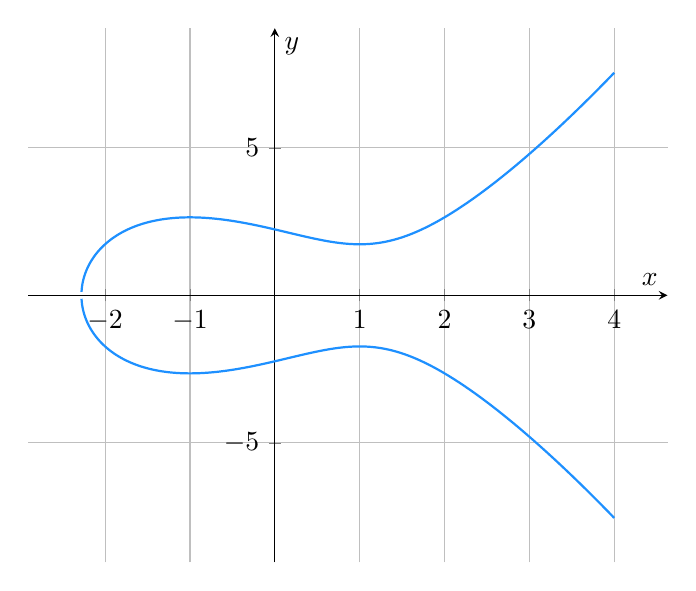
\begin{tikzpicture}
\begin{axis}[
    axis lines=middle, % Axes pass through the origin
    xlabel=$x$,
    ylabel=$y$,
    grid=both,
    enlargelimits=0.1, % Add some padding
    domain=-3:4,    % x-range for the plot
    samples=1300,      % Number of points (for a smooth curve)
    smooth,           % Makes the line smoother
    width=0.8\textwidth
]
% Plot the top half of the curve
\addplot[maincolor, thick] {sqrt(x^3 - 3*x + 5)};

% Plot the bottom half of the curve
\addplot[maincolor, thick] {-sqrt(x^3 - 3*x + 5)};

\end{axis}
\end{tikzpicture}
\end{figure}

L'idea alla base di ECC è quella di \textbf{modulare la curva secondo un numero primo $p$} e di scegliere un punto casuale su di essa, sul quale eseguire una particolare operazione, la \textbf{somma tra punti}, che vedremo con calma, poiché risulta particolarmente complessa.

Ad ogni modo, sia Diffie-Hellman che ECC sfruttano la difficoltà di calcolare il \textbf{logaritmo discreto}. In altre parole, per noi e per i computer è semplice risolvere la seguente equazione:

\begin{equation*}
    2 ^ x = 9
\end{equation*}

Infatti, per risolverlo basta calcolare il logaritmo.

\begin{equation*}
    x = log _ {2} 9
\end{equation*}

\newpage

Il discorso cambia però quando applichiamo questo ragionamento ai moduli (che vedremo meglio in seguito; se non li avete mai visti, potete saltare al prossimo paragrafo). Infatti, se consideriamo un' equazione del genere:

\begin{equation*}
    2 ^ x \equiv 9 \mod 17
\end{equation*}


È complicatissimo risolverla, perché non è più possibile applicare il logaritmo a causa del modulo. Come per la fattorizzazione, ad oggi non esistono algoritmi che permettano di risolvere queste equazioni in tempi ragionevoli.


\subsubsection{Post-Quantum}
Ultimo appunto prima di partire con i cifrari antichi: voglio fare una piccola introduzione sui \textbf{Cifrari Post-Quantum}, perché gli algoritmi \textbf{RSA}, \textbf{Diffie-Hellman} e \textbf{ECC} sono attualmente molto difficili da rompere con i computer moderni, ma è possibile che, con i computer \textbf{quantistici}, possano essere violati anche in pochi secondi. Infatti, i computer quantistici sono particolarmente adatti a risolvere problemi su cui si basano questi algoritmi: ad esempio, possono fattorizzare numeri enormi o calcolare il logaritmo discreto in tempi brevissimi.

Tuttavia, ad oggi i computer quantistici sono ancora in fase di sviluppo e c’è ancora molta strada da fare: per esempio, il numero più grande mai fattorizzato con un computer quantistico è \textbf{21}. Non si può sapere come saranno i computer quantistici in futuro; per questo motivo, i maggiori ricercatori stanno lavorando per creare nuovi cifrari \textbf{difficili da rompere anche per computer quantistici}.

Tra questi, quelli che stanno ricevendo maggiore attenzione dalla comunità scientifica sono i \textbf{Lattice-Based}. Si tratta di algoritmi che sfruttano i \textbf{reticoli} (in inglese \textit{Lattice}), ovvero "piani cartesiani" a n dimensioni, ad esempio $\mathbb{Z} ^ n$.

Si possono generare dei vettori linearmente indipendenti a $n$ dimensioni. A partire da questi, è possibile definire un punto e determinare il percorso più semplice per raggiungerlo usando i nuovi vettori. Ad ogni modo, questi cifrari sono particolarmente complessi, ma rappresentano anche il futuro della crittografia. Per questo motivo, in questo corso non li tratteremo, ma consiglio a tutti di studiarli autonomamente.
























\newpage







\section{Cifrari Antichi - Cesare}

Cominciamo ad analizzare i primi cifrari, iniziando dal più antico mai inventato: infatti, come avevamo già detto nell'introduzione, il \textbf{Cifrario di Cesare} risale all'Impero romano.  
Il cifrario fu ideato per inviare ai legionari informazioni per proseguire la battaglia.  
Chiaramente non potevano mandare i messaggi in chiaro, anche perché, se gli avversari ne venivano a conoscenza, potevano rispondere con una contromossa.  
Per questo \textbf{Giulio Cesare} inventò un cifrario che si basava sullo spostamento di un determinato numero di posizioni delle lettere nell'alfabeto.  
Un classico esempio del cifrario di Cesare è quello di \textbf{spostare di 3 posizioni indietro}.


\begin{figure}[h]
    \centering
    \includegraphics[width=\linewidth]{logos/1_1_cripto.pdf}
\end{figure}


Le lettere che "escono a sinistra" le associamo alle ultime tre lettere.


\begin{figure}[h]
    \centering
    \includegraphics[width=0.8\linewidth]{logos/1_2_cripto.pdf}
\end{figure}

Per cifrare un messaggio basta prendere ogni lettera del testo in chiaro e sostituirla con la lettera corrispondente nella tabella.  
Ad esempio, se volessimo cifrare la parola \textbf{Abbecce}, con il cifrario di Cesare diventerebbe \textbf{Deehffh}.


Per decifrare, invece, basta applicare lo stesso procedimento, ma spostando l'alfabeto verso destra.  
Con questo esempio, il testo decifrato sarà:

\begin{figure}[h]
    \centering
    \includegraphics[width=0.8\linewidth]{logos/1_3_cripto.pdf}
\end{figure}


\newpage

In questo esempio abbiamo spostato l'alfabeto di tre posizioni, ma questo è un numero che possiamo scegliere liberamente.  
Secondo la tradizione, Giulio Cesare utilizzava il numero tre, ma si può scegliere qualsiasi valore di spostamento.  
Poiché questo numero è decisivo per la cifratura, il numero di spostamenti non è altro che la \textbf{chiave} del sistema.  
Chiaramente, a chiavi diverse corrispondono cifrari diversi e, di conseguenza, differenti cifrature dei messaggi.


Una possibile implementazione in Python del cifrario di Cesare con 3 spostamenti:

\begin{lstlisting}[language=Python]
def Cifratura_Cesare(mess):
    return "".join([chr(((ord(char) - ord('a') + 3) % 26) + ord('a')) for a in mess])

def Decifratura_Cesare(mess):
    return "".join([chr(((ord(char) - ord('a') - 3) % 26) + ord('a')) for a in mess])
\end{lstlisting}


Online, questa cifratura viene anche chiamata \textbf{ROT} (abbreviazione di \textit{ROTation}), seguita dal numero di spostamenti.  
Quindi, \textbf{ROT3} corrisponde a 3 spostamenti (come negli esempi precedenti), mentre \textbf{ROT15} sposterà di 15 posizioni.  
In Python, un'implementazione per un generico \textbf{ROT-n} potrebbe essere:


\begin{lstlisting}[language=Python]
def Cifratura_ROTn(mess, n):
    return "".join([chr(((ord(char) - ord('a') + n) % 26) + ord('a')) for a in mess])

def Decifratura_ROTn(mess, n):
    return "".join([chr(((ord(char) - ord('a') - n) % 26) + ord('a')) for a in mess])
\end{lstlisting}




Quindi, se qualcuno vuole usare questo cifrario, basta scegliere un numero tra 1 e 25 e tenerlo segreto.  
Tuttavia, questo metodo è soggetto ad attacchi \textbf{brute-force}: come abbiamo detto, questo cifrario ha al massimo \textbf{25 chiavi possibili}, quindi qualcuno potrebbe creare un programma che provi tutte le combinazioni.  
Un possibile programma in Python:


\begin{lstlisting}[language=Python]
def attacco_rotn(messDaDecifrare):
    for i in range(1, 26):
        print(Decifratura_ROTn(messDaDecifrare, i))
\end{lstlisting}


\newpage

\subsection{Cifrari Monoalfabetici}
In realtà, l'attacco brute-force non è l'unico al quale è soggetto questo cifrario.  
Questo tipo di cifrario è definito \textbf{monoalfabetico} perché la stessa lettera viene sempre cifrata con la stessa lettera corrispondente.  
Tutti i cifrari monoalfabetici sono soggetti ad attacchi detti \textbf{Letter Frequency}.  
Ciò significa che la \textbf{percentuale} di una lettera nel testo originale è la stessa della lettera corrispondente nel testo cifrato.  
Facciamo un esempio con \textbf{Abbcccdddd}, che, cifrato con ROT3, diventa \textbf{Deefffgggg}.

\vspace{0.2cm}
\[
\begin{array}{c@{\hskip 0.1cm}c@{\hskip 0.1cm}c}
  \text{\LARGE Abbcccdddd} & \Longrightarrow & \text{\LARGE Deeffgggg} \\[0.2cm]

  \begin{array}{c|c}
    \textbf{Lettera} & \textbf{percentuale} \\
    \hline
    A & 10\% (1/10) \\
    B & 20\% (2/10) \\
    C & 30\% (3/10) \\
    D & 40\% (4/10) \\
  \end{array}
  &
  &
  \begin{array}{c|c}
    \textbf{Lettera} & \textbf{percentuale} \\
    \hline
    D & 10\% (1/10) \\
    E & 20\% (2/10) \\
    F & 30\% (3/10) \\
    G & 40\% (4/10) \\
  \end{array}
\end{array}
\]

\vspace{0.2cm}
Questa caratteristica dei sistemi monoalfabetici può essere sfruttata per decifrare, anche parzialmente, il messaggio.  
Questo perché possiamo creare delle tabelle con la frequenza di ogni lettera per ciascuna lingua.  
Ad esempio, la \textbf{tabella di frequenza} della lingua italiana è:


\begin{table}[h]
\centering
    \begin{tabular}{cc}
\multicolumn{1}{c|}{Lettera} & Frequenza \\ \hline
\multicolumn{1}{c|}{E}       & 11.49 \%  \\
\multicolumn{1}{c|}{A}       & 10.85 \%  \\
\multicolumn{1}{c|}{I}       & 10.18 \%  \\
\multicolumn{1}{c|}{O}       & 9.97 \%   \\
\multicolumn{1}{c|}{N}       & 7.02 \%   \\
\multicolumn{2}{c}{...}                 
\end{tabular}
\end{table}

\begin{center}
    
link alla tabella completa : \href{https://www.sttmedia.com/characterfrequency-italian}{https://www.sttmedia.com/characterfrequency-italian}
\end{center}

Questa tabella indica che, in media, un messaggio o una parola in italiano ha quelle probabilità di contenere le rispettive lettere.  
Quindi, perché stiamo facendo tutto questo discorso? Perché, se facciamo la stessa analisi anche sul messaggio cifrato e confrontiamo le lettere più frequenti nel messaggio cifrato con la tabella sopra, è possibile identificare alcune lettere.  
Chiaramente, più è lungo il messaggio, più è probabile indovinare le lettere.


\textbf{N.B.} Chiaramente, esistono tabelle di frequenza per ogni lingua; qui ho riportato quella italiana come esempio.

\newpage

Facciamo un esempio pratico: supponiamo di avere il seguente messaggio:
\vspace{0.2cm}

\textit{hlvc irdf uvc crxf uz Tfdf, tyv mfcxv r dvqqfxzfief, kir ulv trkvev efe zekviifkkv uz dfekz, klkkf r jvez v r xfcwz, r jvtfeur uvccf jgfixviv v uvc izvekiriv uz hlvccz, mzve, hlrjz r le kirkkf, r izjkizexvijz, v r giveuvi tfijf v wzxlir uz wzldv, kir le gifdfekfizf r uvjkir, v le’rdgzr tfjkzvir urcc’rckir grikv; v zc gfekv, tyv zmz tfexzlexv cv ulv izmv, gri tyv iveur retfi gzu jvejzszcv rcc’fttyzf hlvjkr kirjwfidrqzfev, v jvxez zc glekf ze tlz zc crxf tvjjr, v c’Ruur izetfdzetzr, gvi izgzxczri gfz efdv uz crxf ufmv cv izmv, rccfekrereufjz uz elfmf, crjtzre c’rthlr uzjkveuvijz v irccvekrijz ze elfmz xfcwz v ze elfmz jvez. }
\vspace{0.2cm}

Possiamo fare un'analisi di frequenza su questo messaggio e confrontarla con la \textbf{tabella di frequenza} della lingua italiana.


\[
\begin{array}{c@{\hskip 1cm}c} % two columns with 1cm space between
% First table (uppercase)

\text{\LARGE Messaggio cifrato} & \text{\LARGE Tabella di frequenza} \\ [0.2cm]

\begin{array}{|c|c|}
\hline
\text{Lettera} & \text{Frequenza} \\ \hline
V & 12.12\%  \\ 
 Z & 11.52\%  \\ 
 R & 9.90\%  \\ 
 F & 9.09\%  \\ 
 E & 8.28\%  \\ 
 I & 7.88\%  \\ 
 C & 6.46\%  \\ 
 K & 5.45\%  \\ 
 U & 4.44\%  \\ 
 J & 4.44\%  \\ 
 L & 4.04\%  \\ 
 T & 3.64\%  \\ 
 X & 2.83\%  \\ 
 G & 2.42\%  \\ 
 D & 2.02\%  \\ 
 M & 1.82\%  \\ 
 H & 1.01\%  \\ 
 W & 1.01\%  \\ 
 Y & 0.81\%  \\ 
 Q & 0.61\%  \\ 
 S & 0.20\%  \\ 
 
\hline
\end{array}
&
% Second table
\begin{array}{|c|c|}
\hline
\text{Lettera} & \text{Frequenza} \\ \hline
E & 11.49\%  \\ 
A & 10.85\%  \\ 
I & 10.18\%  \\ 
O & 9.97\%  \\ 
N & 7.02\%  \\ 
T & 6.97\%  \\ 
R & 6.19\%  \\ 
L & 5.70\%  \\ 
S & 5.48\%  \\ 
C & 4.30\%  \\ 
D & 3.39\%  \\ 
U & 3.16\%  \\ 
P & 2.96\%  \\ 
M & 2.87\%  \\ 
V & 1.75\%  \\ 
G & 1.65\%  \\ 
H & 1.43\%  \\ 
B & 1.05\%  \\ 
F & 1.01\%  \\ 
Z & 0.85\%  \\ 
Q & 0.45\%  \\  
\hline
\end{array}
\end{array}
\]


Con questo, capiamo che molto probabilmente una lettera tra \textbf{V}, \textbf{Z} oppure \textbf{R} nel testo cifrato corrisponderà alla \textbf{E} nel messaggio in chiaro.  
Chiaramente, questo ragionamento si può applicare a tutte le altre lettere, le quali, con buona probabilità, corrisponderanno a una delle lettere con percentuali simili.


\textbf{N.B.} Usando l'alfabeto italiano, le lettere straniere (\textbf{K}, \textbf{J}, \textbf{W}, \textbf{X} e \textbf{Y}) non sono presenti nella tabella di frequenza.  
Nel messaggio cifrato che ho creato, queste lettere possono apparire, ma mancheranno 5 lettere dell'alfabeto italiano perché non hanno corrispondenza con le lettere straniere mancanti.


\newpage
Inoltre, si possono fare delle \textbf{osservazioni linguistiche}.  
Per esempio, in italiano solamente le lettere \textbf{A}, \textbf{E} e \textbf{O} possono stare da sole (per indicare le relative funzioni di preposizione).  
Quindi, nel messaggio cifrato possiamo sicuramente dire che le lettere \textbf{V} e \textbf{R} possono corrispondere solamente a \textbf{A}, \textbf{E} oppure \textbf{O}, il che combacia anche con le percentuali delle tabelle.  
Ad ogni modo, proviamo a sostituire nel messaggio cifrato le lettere con la \textbf{percentuale} più simile:

\vspace{0.2cm}

\textit{hder tivo ser ripo sa tovo, ufe gorpe i vezzopaotno, lti sde uilene non anlettolle
sa vonla, ldllo i cena e i porba, i ceuonsi serro cmotpete e ser taenltite sa hderra,
gaen, hdica i dn ltillo, i tacltanpetca, e i mtenset uotco e bapdti sa badve, lti dn
mtovonlotao i seclti, e dn’ivmai uoclaeti sirr’irlti mitle; e ar monle, ufe aga uonpadnpe
re sde tage, mit ufe tensi inuot mas cencaqare irr’ouufao hdecli lticbotvizaone, e cepna
ar mdnlo an uda ar ripo uecci, e r’rssi tanuovanuai, met tamaprait moa nove sa ripo soge
re tage, irronlininsoca sa ndogo, ricuain r’iuhdi saclensetca e tirrenlitca an ndoga
porba e an ndoga cena.}
\vspace{0.2cm}

Ora, come ora, il testo non sembra molto chiaro, ma possiamo iniziare a sistemarlo.  
Per esempio, come dicevamo prima, le lettere singole possono essere solamente \textbf{E}, \textbf{A} o \textbf{O}.  
Attualmente, però, abbiamo \textbf{I} e \textbf{E}, quindi dobbiamo sostituire la \textbf{I}.  
Poiché la \textbf{I} è molto vicina in percentuale (secondo la tabella di frequenza) alla \textbf{A}, proviamo a invertire le due lettere.  
In questo modo, il testo diventa:

\vspace{0.2cm}
\textit{hder tavo ser rapo si tovo, ufe gorpe \textcolor{red}{a} vezzopiotno, lta sde ualene non inlettolle
si vonli, ldllo \textcolor{red}{a} ceni e \textcolor{red}{a} porbi, \textcolor{red}{a} ceuonsa serro cmotpete e ser tienltate si hderri, [...]}
\vspace{0.2cm}

Ora possiamo notare che ci sono molti \textbf{SI}, che molto probabilmente possono essere \textbf{DI}.  
Quindi, proviamo a invertire \textbf{D} e \textbf{S}.

\vspace{0.2cm}
\textit{hser tavo der rapo \textcolor{red}{d}i tovo, ufe gorpe a vezzopiotno, lta dse ualene non inlettolle
\textcolor{red}{d}i vonli, lsllo a ceni e a porbi, a ceuonda derro cmotpete e der tienltate \textcolor{red}{d}i hserri, [...]}\vspace{0.2cm}

Ora siamo abbastanza sicuri che le lettere \textbf{D}, \textbf{A}, \textbf{I} e \textbf{E} siano al posto corretto.  
Possiamo continuare a fare delle analisi e, man mano, dedurre il testo originale.  
Per esempio, nella prima riga c'è \textbf{DSE}, che molto probabilmente potrebbe essere \textbf{DUE} (visto che la \textbf{D} e la \textbf{E} siamo sicuri che siano corrette).  
Oppure, la parola \textbf{vezzopiotno} potrebbe essere \textbf{mezzogiorno}, e così via.  
Se vuoi, puoi provare a risolvere questo enigma da solo, ho creato un codice Python: 


\sloppy
link: \textcolor{maincolor}{\url{https://github.com/AlexBro98LoVero/Dispense/blob/main/Giochi/1_1_giocoParole.py}}

altrimenti, continua che ora c'è la soluzione.

\newpage
Ad ogni modo, con un po' di pazienza potreste vedere che il testo cifrato qui sopra non è altro che i primi versi dei \textbf{Promessi Sposi}.

\vspace{0.2cm}
\textit{quel ramo del lago di como, che volge a mezzogiorno, tra due catene non interrotte di monti, tutto a seni e a golfi, a seconda dello sporgere e del rientrare di quelli, vien, quasi a un tratto, a ristringersi, e a prender corso e figura di fiume, tra un promontorio a destra, e un’ampia costiera dall’altra parte; e il ponte, che ivi congiunge le due rive, par che renda ancor piu sensibile all’occhio questa trasformazione, e segni il punto in cui il lago cessa, e l’adda rincomincia, per ripigliar poi nome di lago dove le rive, allontanandosi di nuovo, lascian l’acqua distendersi e rallentarsi in nuovi golfi e in nuovi seni. }
\vspace{0.2cm}


\textbf{N.B.} Per semplicità, ho messo tutto in minuscolo e ho rimosso le lettere accentate, ma chiaramente, se contemplate, possono essere d'aiuto per scoprire parole all'interno del testo.

\vspace{0.2cm}

Ora vediamo quanto erano corrette le corrispondenze.


\begin{figure}[h]

    \centering
    \includegraphics[width=\linewidth]{logos/1_5_cripto.pdf}

\end{figure}

Si può notare che, nel complesso, questa tecnica ha indovinato quasi tutte le lettere; infatti, molte erano sbagliate di una sola posizione.

\begin{itemize}
    \item Indovinate: 4/21 $\approx$ 19.0 \%
    \item Sbagliato di una casella: 10/21 $\approx$ 47.6 \%
    \item Sbagliato di due caselle: 5/21 $\approx$ 23.8 \%
    \item sbagliato di tre caselle: 1/21 $\approx$ 4.8 \%
    \item sbagliato di quattro caselle: 1/21 $\approx$ 4.8 \%
\end{itemize}























\section{Cifrati Antichi - Enigma}

\begin{wrapfigure}{r}{0.35\textwidth}
    \centering
    \includegraphics[width=0.30\textwidth]{logos/2_1cripto.jpg}
    \caption*{Foto della macchina Enigma}
\end{wrapfigure}

La tecnica \textbf{OTP}, per come l'abbiamo studiata fino ad ora, è utilizzabile solo tramite i computer, ma in realtà è molto più antica e, durante la \textbf{Seconda Guerra Mondiale}, ha giocato un ruolo fondamentale. Infatti, i tedeschi hanno utilizzato la \textbf{Macchina Enigma}, che permetteva loro di comunicare inviando messaggi cifrati. La macchina Enigma, per l'appunto, usa una tecnica di crittografia molto simile, se non uguale, all'\textbf{OTP}.


\subsection{Preambolo Storico}

La macchina Enigma è stata brevettata da \textbf{Arthur Scherbius}, un ingegnere tedesco, nel \textbf{1918}. Al contrario di quanto si pensa, Enigma veniva utilizzata anche prima della Seconda Guerra Mondiale, soprattutto dalla \textbf{marina militare tedesca}. Tuttavia, Enigma ha avuto un ruolo importantissimo durante la Seconda Guerra Mondiale, perché ha permesso ai tedeschi di inviare messaggi sicuri, impedendo agli Alleati di comprendere le decisioni militari tedesche. 

La macchina Enigma aveva una \textbf{chiave privata} (che vedremo in dettaglio più avanti) che veniva cambiata \textbf{ogni giorno a mezzanotte}. La chiave veniva inviata soltanto agli ufficiali tedeschi di grado più alto per evitare fughe di informazioni riservate. Infatti, verso mezzanotte, ai generali tedeschi arrivava un messaggio chiamato \textbf{Schlüsselheft}, che conteneva la chiave del giorno. In realtà, alcuni reparti tedeschi, come la marina militare, che richiedevano maggiore sicurezza, cambiavano chiave ogni \textbf{8 ore}. Inoltre, erano previsti protocolli di sicurezza, come il fatto che il \textbf{Schlüsselheft} dovesse essere conservato in un luogo sicuro sotto chiave, con accesso riservato solo a poche persone autorizzate. Se vi era il rischio che gli Alleati potessero entrarne in possesso, il \textbf{Schlüsselheft} doveva essere immediatamente distrutto tramite il fuoco.

\subsection{Funzionamento}

La macchina Enigma serviva per crittografare e decrittografare i messaggi. Era dotata di una tastiera e, alla pressione di un tasto (dove ogni tasto rappresentava una lettera dell'alfabeto tedesco), si accendeva un led che indicava un'altra lettera dell'alfabeto. Per utilizzare una macchina Enigma, di solito erano necessarie due persone: una che scriveva il messaggio da cifrare o decifrare e un'altra che annotava le lettere che si illuminavano.

\begin{wrapfigure}{l}{0.35\textwidth}
    \centering
    \vspace{-1.5cm}
    \includegraphics[width=0.35\textwidth]{logos/2_2cripto.jpg}
\end{wrapfigure}

\vspace{+1.5cm}

Nell'immagine possiamo notare che, alla pressione del tasto \textbf{I} sulla tastiera, si illumina la lettera \textbf{U} nella parte superiore.

\afterpage{\clearpage}



\newpage
\subsection{Struttura}

Ogni macchina Enigma era composta da sei parti principali: \textbf{Tastiera}, \textbf{Rotori}, \textbf{Riflettore}, \textbf{Lampboard}, \textbf{Plugboard} e la \textbf{Batteria}.  

Partiamo dagli elementi più semplici: la batteria serviva ad alimentare la parte elettrica della macchina, mentre la tastiera conteneva le 26 lettere dell'alfabeto sotto forma di pulsanti. La tastiera funzionava in modo simile a quelle odierne, nel senso che, alla pressione di un tasto, si chiudeva il circuito elettrico.  

La \textbf{Lampboard} (detta \textbf{Lampenbrett} in tedesco) era la parte in cui si trovavano le lettere che si illuminavano alla pressione dei tasti sulla tastiera.  

\subsubsection{Plugboard}

La \textbf{Plugboard} (detta anche \textbf{Steckerbrett}) serviva per invertire una coppia di lettere. Questa inversione avveniva sia in input (quindi prima di eseguire l'algoritmo di cifratura) sia in output (dopo aver cifrato il messaggio). Questa caratteristica serviva esclusivamente ad aggiungere un ulteriore livello di sicurezza, ma non era il punto focale della macchina.

\begin{figure}[h]
    \centering
    \includegraphics[width=0.6\linewidth]{logos/2_3cripto.jpg}
\end{figure}

Nell'immagine possiamo notare come siano collegate le coppie (\textbf{A}, \textbf{J}) e (\textbf{S}, \textbf{O}).  
Quindi, se veniva premuto il tasto \textbf{A} sulla tastiera, esso veniva prima trasformato in \textbf{J}, che poi seguiva il resto dell'algoritmo.  
Allo stesso modo, se la lettera crittata era \textbf{S}, questa veniva cambiata in \textbf{O}, e quindi si illuminava la lettera \textbf{O} sulla lampboard.

\subsubsection{Rotori}

\begin{wrapfigure}{r}{0.35\textwidth}
    \vspace{-1cm}
    \centering
    \includegraphics[width=0.35\textwidth]{logos/2_4cripto.png}
    \caption*{Render 3D di tre rotori collegati}
\end{wrapfigure}

La parte principale dell'algoritmo di cifratura sono \textbf{i rotori}, che permettono di trasformare le lettere per crittarle.  
Un rotore è un componente metallico circolare collegato a un ingranaggio che gli permette di ruotare e cambiare lettera, come vedremo in seguito.  
Inoltre, è montato su un asse che ne consente la rotazione e, su entrambi i lati, presenta 26 punti di contatto metallici che permettono di trasmettere la corrente tra un rotore e l'altro.

\afterpage{\clearpage}   


\newpage
Per comprendere meglio il funzionamento di un rotore, è utile analizzarne la struttura interna:

\begin{figure}[h]
    \centering
    \includegraphics[width=0.6\linewidth]{logos/2_5cripto.pdf}
\end{figure}

Come accennato in precedenza, entrambi i lati del rotore presentano piastre metalliche per la conduzione della corrente (indicate dalla freccia rossa nell'immagine). Inoltre, ogni punto di contatto su un lato è collegato a un punto sull'altro lato, ma in modo disordinato. Questo collegamento permette di mescolare le lettere: una lettera che "entra" nel rotore ne "uscirà" come un'altra, a causa di questo rimescolamento.  

Di norma, una macchina Enigma contiene tre rotori collegati in serie per aumentare la complessità della cifratura. Tuttavia, alcune versioni della macchina Enigma utilizzano quattro o più rotori, semplicemente per incrementare la sicurezza e rendere ancora più difficile la decrittazione.





\subsubsection{Riflettore}
\begin{wrapfigure}{r}{0.35\textwidth}
    \vspace{-1cm}
    \centering
    \includegraphics[width=0.35\textwidth]{logos/2_6cripto.png}
    \caption*{Render 3D di un Riflettore}
\end{wrapfigure}

Per aumentare ulteriormente la sicurezza, i tre rotori sono collegati a un \textbf{Riflettore}, il quale fa "rientrare" il segnale nei rotori, permettendo un'ulteriore trasformazione delle lettere. Questo avviene perché la corrente attraversa nuovamente tutti e tre i rotori in senso inverso.

In questo modo, una lettera viene cifrata \textbf{sei volte} prima di essere visualizzata sulla lampboard.

\afterpage{\clearpage}  


\newpage
\subsection{Funzionamento}
Ripercorriamo il funzionamento della macchina Enigma. 

\begin{figure}[h]
    \centering
    \includegraphics[width=0.9\linewidth]{logos/2_7cripto.pdf}
\end{figure}

Quando viene premuto un tasto sulla \textbf{Tastiera}, il segnale passa attraverso la \textbf{Plugboard}, che sostituisce la lettera con quella associata se un cavo è collegato; altrimenti, il segnale prosegue direttamente verso i \textbf{Rotori}. Successivamente, attraversa i tre rotori, modificando la lettera tre volte. Grazie al \textbf{Riflettore}, il segnale viene reinviato attraverso i rotori, che trasformano nuovamente la lettera per altre tre volte. Infine, il segnale passa nuovamente per la \textbf{Plugboard}, che può applicare un'ulteriore sostituzione se la lettera è collegata a un'altra. Dopo tutte queste trasformazioni, la lettera finale viene visualizzata sulla \textbf{Lampboard}. 

Durante questo processo, la lettera viene trasformata un minimo di \textbf{6 volte} e fino a un massimo di \textbf{8 volte} se la \textbf{Plugboard} modifica sia l'input che l'output.

Non appena il tasto premuto viene rilasciato, il primo rotore ruota di una posizione grazie a un ingranaggio, modificando così la configurazione delle lettere. Questo meccanismo assicura che, anche premendo due volte di seguito la stessa lettera, vengano visualizzate lettere completamente diverse, poiché la rotazione del rotore cambia continuamente le combinazioni possibili. 

\begin{figure}[h]
    \centering
    \includegraphics[width=\linewidth]{logos/2_8cripto.pdf}
\end{figure}

























\section{One Time Pad}
La prima forma di crittografia che vediamo è \textbf{One Time Pad}, che è una crittografia \textbf{Simmetrica}. Con il termine crittografia simmetrica si intendono tutte le tecnite crittografiche che usano una sola chiave per criptare e decriptare, al contrario della crittografia asimmetrica che ne usa due, ma questo lo vedremo bene più avanti. Prima di capire bene il funzionamento di questa tecnica è meglio rivedere cos'è lo \textbf{XOR} e come funziona.


\subsection{XOR}
Lo \textbf{XOR} (\textit{eXclusive OR}) è un operatore booleano binario la cui tabella di verità è la seguente:

\begin{center}
\begin{table}[h]
\centering
\begin{tabular}{c|c|c}
A & B & XOR(A, B) \\
\hline
0 & 0 & 0         \\
0 & 1 & 1         \\
1 & 0 & 1         \\
1 & 1 & 0         \\
\end{tabular}
\end{table}
\end{center}

Per ricordarla a memoria, basta sapere che, se A e B sono diversi, lo XOR restituisce 1; altrimenti, se sono uguali, restituisce 0.

Ci interessano in particolare le seguenti proprietà dello XOR:

\begin{equation*} (A \oplus B) \oplus B = A \end{equation*}

\begin{equation*} A \oplus 0 = A \end{equation*}

dove $\oplus$ è il simbolo dello XOR. In realtà, queste proprietà sono tutto ciò che ci serve per comprendere il nostro algoritmo crittografico, quindi passiamo ad analizzarne il funzionamento.

\newpage
\subsection{Funzionamento}
L'algoritmo \textbf{OTP} inizia generando una chiave lunga almeno quanto il messaggio da cifrare. La chiave può assumere qualsiasi forma, purché sia privata e nessuno la conosca. Dopo la generazione della chiave, è sufficiente XORarla con il messaggio che vogliamo inviare:  

\begin{equation*}
    C = M \oplus K 
\end{equation*}

dove \(C\) è il messaggio cifrato (\textit{Crypted message}), \(M\) è il messaggio originale (\textit{Message}) e \(K\) è la chiave (\textit{Key}).  

Una volta inviato il messaggio, il destinatario può semplicemente applicare l'operazione XOR tra il messaggio ricevuto e la chiave per recuperare il messaggio originale:  

\begin{equation*}
   C \oplus K
\end{equation*}

Per capire perché il metodo funziona, sostituiamo l'equazione precedente (\(C = M \oplus K\)):  

\begin{equation*}
    (M \oplus K) \oplus K
\end{equation*}

Utilizzando la proprietà dello XOR, otteniamo:  

\begin{equation*}
    M = (M \oplus K) \oplus K 
\end{equation*}

In questo modo, applicando l'operazione XOR, recuperiamo esattamente il messaggio originale.  














\begin{figure}[h]
    \centering
    \includegraphics[width=0.9\linewidth]{logos/3_1cripto.pdf}
\end{figure}


\subsubsection{Considerazioni}

Questo algoritmo, però, non si occupa della condivisione sicura della chiave. Per questo scopo si può utilizzare l'algoritmo \textbf{Diffie-Hellman}, che è progettato proprio per condividere chiavi private in modo sicuro.  

La forza e la bellezza di questo algoritmo risiedono nel fatto che è \textbf{completamente sicuro}: è stato infatti dimostrato matematicamente che è impossibile decifrare il messaggio cifrato (\(M \oplus K\)) senza conoscere la chiave. L'\textbf{OTP} è, infatti, l'unico algoritmo \textbf{impossibile da decifrare} e completamente sicuro che conosciamo al momento. L'unico metodo per indovinare il messaggio è tentare casualmente e sperare in un colpo di fortuna.  

Ovviamente, non è tutto oro ciò che luccica: se fosse davvero perfetto, useremmo solo questa tecnica e saremmo al 100\% sicuri. Tuttavia, come vedremo, questo algoritmo presenta un problema non da poco.  




\subsection{Crackabilità}
Il problema di questa tecnica risiede nel nome: \textbf{ONE TIME Pad}. Ovvero, questa tecnica si può usare \textbf{una sola volta} con la stessa chiave. Questo è un requisito fondamentale, perché qualora una chiave venga usata più di una volta, tramite varie tecniche si può estrapolare la chiave e i messaggi, almeno parzialmente.  

Questo accade perché, dati due messaggi in chiaro (\(\mathbf{M_1}\), \(\mathbf{M_2}\)), una chiave privata (\(\mathbf{K}\)) e le loro combinazioni cifrate (\(\mathbf{C_1}\), \(\mathbf{C_2}\)):  

\begin{equation*}
    C_1 = M_1 \oplus K 
\end{equation*}
\begin{equation*}
    C_2 = M_2 \oplus K    
\end{equation*}

Supponiamo di aver intercettato i messaggi cifrati: possiamo applicare l'operazione XOR tra di loro:  

\begin{equation*}
    C_1 \oplus C_2
\end{equation*}

Riscriviamo l'espressione sostituendo i valori di \(C_1\) e \(C_2\):  

\begin{equation*}
    C_1 \oplus C_2 = (M_1 \oplus K ) \oplus (M_2 \oplus K)
\end{equation*}

Ora, grazie alla proprietà associativa dello XOR, possiamo riorganizzare i termini:  

\begin{equation*}
    C_1 \oplus C_2 = (M_1 \oplus M_2 ) \oplus (K \oplus K)
\end{equation*}

Poiché \(K \oplus K = 0\), otteniamo:  

\begin{equation*}
    C_1 \oplus C_2 = (M_1 \oplus M_2 ) \oplus 0
\end{equation*}

Infine, ricordando che \(X \oplus 0 = X\), il risultato finale è:  

\begin{equation*}
    C_1 \oplus C_2 = M_1 \oplus M_2 
\end{equation*}




Dopo tutti questi passaggi, abbiamo scoperto che la XOR tra i du.



e messaggi cifrati è uguale alla XOR dei due messaggi in chiaro. In questo modo, siamo riusciti a "rimuovere" la chiave. Chiaramente, con la XOR dei messaggi in chiaro, comunque non riusciamo a decriptarli, ma possiamo dedurre alcune parti. Infatti, esistono alcuni algoritmi, come \textbf{crib drag}, che, dati alcuni messaggi cifrati, possono decifrare parti dei messaggi e della chiave. Questi algoritmi sono particolarmente complessi e sfruttano certi pattern nelle frasi (come banalmente gli spazi, oppure gli articoli nelle varie lingue) e anche degli \textbf{attacchi con dizionario} (dictionary attack). Per capirli bene e in maniera pratica, consiglio di scaricare i seguenti script Python: \textcolor{maincolor}{\url{https://github.com/CameronLonsdale/MTP}}. Inoltre, per gli amanti del rap, vi lascio un esempio divertente per cercare di capire quale canzone è: \textcolor{maincolor}{\url{https://github.com/AlexBro98LoVero/Dispense/blob/main/Giochi/3_1_mtptxt}}













\newpage

\section{Stream}

Il prossimo algoritmo che vedremo è quello degli \textbf{Stream}.  
Prima di parlarne, però, dobbiamo capire cosa sono i \textbf{Pseudo-Random Number Generator}, perché sono la base degli stream, anche se inizialmente possono sembrare non avere nulla a che fare con essi.

\subsection{PRNG}

Per chi ha già creato qualche programma in \textbf{C}/\textbf{C++}, può darsi che abbia dovuto \textbf{generare dei numeri casuali}.  
Tuttavia, è difficile crearli perché i computer sono sistemi \textbf{deterministici}, cioè ad ogni input corrisponde sempre lo stesso output.  
Quindi, per i computer è impossibile generare numeri realmente casuali; per questo motivo sono stati inventati gli \textbf{Pseudo-Random Number Generator}, ovvero dei generatori di numeri \textbf{pseudo-casuali}, che a noi \textbf{sembrano} casuali, ma che in realtà sono deterministici.


Un primo esempio è il \textbf{Linear Congruential Generator} (\textit{LCG}), che parte da alcuni valori iniziali $X_0$, $a$, $c$ e $m$ ($X_0$ è detto \textbf{seme} o \textbf{seed}), i quali possono essere scelti a piacere.  
A partire da questi valori, possiamo generare nuovi numeri pseudo-casuali con la seguente formula:


\begin{equation*}
    X_{n+1} = aX_n + c \pmod{m}
\end{equation*}

Per chi non lo sapesse, il simbolo $\pmod{n}$ indica il \textbf{resto della divisione} tra due numeri.  
Per esempio, $9 \pmod{4}$ significa che devo fare la divisione $9/4$ e considerare solo il resto.  
In questo caso, $9/4 = 2$ con resto $1$, quindi $9 \pmod{4} = 1$.  
Riprenderemo questi concetti nei capitoli dedicati a \textbf{RSA} e \textbf{Diffie-Hellman}.


Per esempio, se scegliamo come valori iniziali $m = 9$, $a = 4$, $c = 1$ e come seme $X_0 = 3$, otteniamo la seguente sequenza di numeri pseudo-casuali:


\begin{align*}
    %X_1 &= 4 \cdot X_0 + 1 \pmod{9} \\
    X_1 &= 4 \cdot 3 + 1 \pmod{9} \\
        &= 13 \pmod{9} \\
    X_1  &= 4
    \\
    \\
    X_2 &= 4 \cdot X_1 + 1 \pmod{9} \\
        &= 4 \cdot 4 + 1 \pmod{9} \\
        &= 17 \pmod{9} \\
    X_2 &= 8 
    \\
    \\
    X_3 &= 4 \cdot 8 + 1 \pmod{9} \\
        &= 33 \pmod{9} \\
    X_3 &= 6
\end{align*}

Per questa configurazione, i primi valori generati dalla sequenza sono:

\begin{equation*}
    4, 8, 6, 7 ,2, 1, 5, 3, 4 ... 
\end{equation*}

Si nota che, all'apparenza, sembra una sequenza casuale di numeri, ma in realtà deriva da una formula e da alcune variabili fissate inizialmente ($a$, $m$, $c$ e $X_0$).

Un problema di questi generatori è che sono \textbf{ciclici}, nel senso che, prima o poi, la sequenza si ripete.  
Per esempio, se continuiamo la sequenza di prima:


\begin{equation*}
    \underline{4, 8, 6}, 7, 2, 0, 1, 5, 3, \underline{4, 8, 6}, 7, 2, 0, 1, 5, 3, \underline{4, 8}
\end{equation*}


Notiamo che questa sequenza è lunga 8 numeri, perché poi si ripete.  
Questo problema è dovuto al fatto che abbiamo scelto numeri \textbf{piccoli}; se invece scegliamo numeri più grandi, ad esempio a 10 o 15 cifre, la ciclicità sarà molto più ampia.


Questo sistema di generazione, però, ha un altro problema: dati alcuni output, è possibile ricavare i parametri ($a$, $m$ e $c$).  
Infatti, se prendiamo quattro numeri \textbf{successivi}, che chiamiamo $X_{\alpha}$, $X_{\alpha+1}$, $X_{\alpha+2}$ e $X_{\alpha+3}$, possiamo metterli a sistema.


\begin{equation*}
    \begin{cases}
        X_{\alpha+1} = aX_{\alpha} + c \pmod{m} \\
        X_{\alpha+2} = aX_{\alpha+1} + c \pmod{m} \\
        X_{\alpha+3} = aX_{\alpha+2} + c \pmod{m}
    \end{cases}
\end{equation*}


In questo caso, notiamo che abbiamo un sistema di 3 equazioni con 3 incognite, quindi possiamo risolverlo e calcolare $a$, $m$ e $c$.  
In realtà, il fatto che ci sia il modulo rende tutto più complicato, ma comunque è possibile risolverlo.


Se vi state chiedendo perché è un enorme problema poter dedurre i parametri, la risposta è la seguente: per quanto vedremo tra poco con gli \textbf{stream}, è obbligatorio che la sequenza sia imprevedibile, perché quei numeri saranno le \textbf{chiavi private} per gli stream.  
Pertanto, è necessario che sia impossibile generare le chiavi successive (ovvero i numeri successivi nella sequenza).


Per giocare un po' con il \textbf{LCG}, vi fornisco due link: uno per generare la sequenza di numeri e un altro link che, dati 4 output, calcola $a$, $m$ e $c$.


\vspace{0.2cm}
link sequenza: \textcolor{maincolor}{\url{https://github.com/AlexBro98LoVero/Dispense/blob/main/Giochi/4_1_generaSequenza.py}}

link 4 output: \textcolor{maincolor}{\url{https://github.com/AlexBro98LoVero/Dispense/blob/main/Giochi/4_2_trovareParametri.py}}
\vspace{0.2cm}

\textbf{N.B.} Può succedere che si trovino più parametri validi; questo è dovuto al fatto che si tratta di equazioni modulari.  
Chiaramente, per scoprire quali sono i parametri corretti, bisognerebbe avere altri output e verificare per quali parametri funzionano.


Il \textbf{LCG} era utilizzato fino a \textbf{Java 17} (anno di pubblicazione 2020) come metodo per generare numeri nella libreria standard.

\newpage

\subsection{LFSR}

Un'altra tecnica per generare numeri casuali è quella del \textbf{Linear Feedback Shift Register} (\textit{LFSR}).  
Questo metodo parte definendo un \textbf{registro}, ovvero un \textbf{array} o \textbf{buffer} di bit, inizializzati a un \textbf{valore iniziale}, che fungerà da \textbf{chiave privata} del nostro sistema.  
La lunghezza del registro è arbitraria, ma di solito è di \textbf{32 bit} oppure \textbf{64 bit}.


\begin{figure}[h]
    \centering
    \includegraphics[width=0.7\linewidth]{logos/4_3cripto.pdf}
\end{figure}

Poi si scelgono dei \textbf{tap}, ovvero delle posizioni del buffer.  
Ad esempio, supponiamo di scegliere le posizioni \textbf{2}, \textbf{3} e \textbf{5}. Il numero di tap può variare.  
Queste posizioni saranno usate perché i bit in quelle posizioni verranno \textbf{xorati} tra loro; il risultato andrà in testa al registro e tutti i bit verranno spostati verso destra (e l'\textbf{ultimo} bit andrà perso).


Per esempio, supponiamo di avere un registro a 8 bit con il seguente stato iniziale:


\begin{figure}[h]
    \centering
    \includegraphics[width=0.7\linewidth]{logos/4_4cripto.pdf}
\end{figure}

Supponiamo che i \textbf{tap} siano: \textbf{2}, \textbf{3} e \textbf{5}.  
Allora, il numero successivo sarà dato dallo \textbf{xor} di questi tre bit.


\begin{center}
    nuovo bit = bit posizione 2 $\oplus$ bit posizione 3 $\oplus$ bit posizione 5 \\
    nuovo bit = 1 $\oplus$ 0 $\oplus$ 0 \\
    nuovo bit = 1
\end{center}

Ora, spostiamo tutti i bit di una posizione verso destra nel registro.


\begin{figure}[!h]
    \centering
    \includegraphics[width=0.7\linewidth]{logos/4_5cripto.pdf}
\end{figure}

Il bit che "sporge" a destra può essere escluso, e in prima posizione inseriamo il bit che abbiamo calcolato in precedenza.


\begin{figure}[!h]
    \centering
    \includegraphics[width=0.7\linewidth]{logos/4_6cripto.pdf}
\end{figure}

E questo sarà il nuovo numero casuale, se ne volessi altri basta rieseguire il procedimento su questo nuovo stato del registro.

\newpage

Una cosa interessante è notare che i \textbf{tap} possono essere espressi come \textbf{polinomi}.  
Rimanendo con l'esempio di prima dei tap (\textbf{2}, \textbf{3}, \textbf{5}), possiamo esprimere questa configurazione tramite il seguente polinomio:


\begin{equation*}
    p(x) = x^2 + x^3 + x^5 +1
\end{equation*}

Qualsiasi configurazione è esprimibile tramite un polinomio, dove i gradi della variabile $x$ corrispondono ai tap, con l'aggiunta di un termine noto ($+1$), e tutti i monomi hanno coefficiente 1.


Questo polinomio ha permesso di studiare le configurazioni ottimali per ottenere una generazione di numeri migliore.  
Infatti, grazie alla rappresentazione polinomiale, si è scoperto che se il polinomio è \textbf{primitivo modulo 2}, la generazione di numeri pseudo-casuali sarà massima.  
Non entrerò nei dettagli, ma considerate che un polinomio primitivo modulo 2 è simile a un \textbf{numero primo}, nel senso che non esistono prodotti di polinomi modulo 2 che diano come risultato quel polinomio primitivo.


Per esempio, il polinomio $p(x) = x^2 + x + 1$ è primitivo, perché non può essere scritto come prodotto di altri polinomi.  
Invece, il polinomio $p(x) = x^2 + 1$ non è primitivo, perché, in modulo 2, può essere scritto come:


\begin{align*}
    p(x) &= (x+1)^2 \pmod{2} \\ 
         &= x^2 + 2x +1 \pmod{2} \\
         &= x^2 +1 \pmod{2}
\end{align*}

Inoltre, sempre con questo meccanismo, la generazione sarà massima anche quando le posizioni sono \textbf{numeri primi tra loro} e quando il \textbf{numero di posti è pari}.


Se non avete compreso bene questa parte, non preoccupatevi: il bello di questo concetto è vedere come una rappresentazione polinomiale di un sistema possa aiutare a migliorarlo e a massimizzarne l'efficienza.


Grazie a questi accorgimenti, si è scoperto che il polinomio più sicuro per un LFSR a 16 bit è:

\begin{equation*}
    p(x) = x^{11} +x^{13} + x^{14} + x^{16} +1
\end{equation*}

\newpage

\subsection{Stream} 

Fatta la premessa sui \textbf{PRNG}, capiamo cosa sono gli stream.  
Gli stream cercano di replicare la forza della cifratura \textbf{OTP}, che, come abbiamo già visto, è l'unico sistema teoricamente impossibile da decifrare.  
In pratica, gli stream utilizzano un algoritmo \textbf{PRNG}, come \textbf{LCG} o \textbf{LFSR} che abbiamo visto prima, e ogni lettera del messaggio viene cifrata tramite una \textbf{cifratura OTP} (cioè mediante un'operazione \textbf{XOR}) con uno dei numeri generati dal PRNG.

Quindi, per cifrare con gli stream, si inizia generando una sequenza di numeri:

\begin{figure}[h]
    \centering 
    \includegraphics[width=0.8\linewidth]{logos/4_1cripto.pdf}
\end{figure}

Successivamente, ogni lettera del messaggio da cifrare viene combinata tramite un'operazione \textbf{XOR} con uno dei numeri generati.

\begin{figure}[h]
    \centering
    \includegraphics[width=0.8\linewidth]{logos/4_2cripto.pdf}
\end{figure}


\textbf{N.B.} Ricordo che il simbolo $\oplus$ indica l'operazione di \textbf{XOR}.


Cosi la stringa "\textbf{parola}" è diventata "\textbf{mK7q\#9}".

Per decifrarlo, sarà sufficiente rigenerare i numeri usando gli stessi parametri e lo stesso seed della cifratura; successivamente, basta eseguire nuovamente l'operazione \textbf{XOR} tra il messaggio cifrato e la chiave, proprio come avviene nella cifratura \textbf{OTP}.

La \textbf{chiave privata} di questo sistema è quindi il \textbf{seed} e i \textbf{parametri} del PRNG, perchè avendoli si può generare la sequenza di numeri e poi cifrare il messaggio. Anche se in realtà si possono rendere pubblici i parametri e lasciare \textbf{solamente il seed come chiave privata}, tanto con valori di paramentri molto altri (10/15 cifre) non rendono facilmente la rottura del cifrario


L'idea alla base degli stream è di replicare la sicurezza dell'\textbf{OTP} e di usare chiavi diverse per ogni cifratura, poiché ricordiamo che il problema dell'OTP è che non si può riutilizzare la stessa chiave, altrimenti si può risalire ai messaggi originali.


Ad oggi, però, i cifrari a \textbf{stream} non sono molto diffusi, a causa della difficoltà di generare numeri veramente casuali e perché, se si scopre il \textbf{seed} (che costituisce la chiave privata del cifrario), è possibile ricavare l'intero messaggio.









\end{document}